% Final
\section{Implementace funkcí}

% Final
V této podkapitole podrobněji popíšu implementaci vybraných funkcí této aplikace. Nejprve popíšu implementaci nové struktury učení, která zásadně mění způsob učení a opakování látky v aplikaci. Této funkci se budu věnovat nejpodrobněji, protože se jedná o nejvýznamnější část celé aplikace. Dále popíšu implementaci registrace a přihlašování pomocí účtu Google, díky čemuž mohou uživatelé získat snadnější přístup do aplikace. Dále popíšu, jakým způsobem jsem z webové aplikace vytvořil progresivní webovou aplikaci, kterou si mohou uživatelé stáhnout a nainstalovat na svá zařízení. Nakonec popíšu implementaci push notifikací, díky kterým mohou být uživatelé lépe informováni o událostech v aplikaci.

% Final
\subsection{Nová struktura učení}

% Final
Se změnou domény aplikace bylo třeba zásadně změnit strukturu učení a opakování látky. Původní aplikace byla zaměřena převážně na zkoušení uživatele z dané látky pomocí cvičení. Aplikace tak při učení neposkytovala uživateli srozumitelné vysvětlení látky. Se změnou domény ovšem vznikla potřeba zavést do učení jasné a srozumitelné vysvětlování látky v průběhu učení. Z tohoto důvodu bylo třeba zásadně změnit model učení, kterému se budu věnovat v následujících částech textu. 

% Final
\subsubsection{Lekce, atomy a bloky učení}

% Final
Základním prvkem učení nového modelu je \texttt{Atom}, který reprezentuje konkrétní znalost nebo koncept, který se uživatel může naučit. Každá lekce je tvořena jedním nebo více atomy. Ke každému atomu je pak přiřazen jeden nebo více tzv. \texttt{StudyBlock} bloků. Každý blok reprezentuje jednu stránku v rámci učení. Na této stránce je uživateli buď vysvětlena nová látka, nebo je uživatel vyzkoušen z dané látky pomocí cvičení. 

% Final
\texttt{StudyBlock} bloky se dělí do dvou typů. \texttt{ExplanationStudyBlock} slouží k vysvětlení nové látky pomocí krátkých videí a animací. \texttt{ExerciseStudyBlock} dále slouží k procvičení dané látky pomocí interaktivních cvičení. Popsaný model je vyobrazen na diagramu \ref{fig:study-model}. Pro zachování přehlednosti jsem do diagramu zahrnul pouze atributy, které jsou relevantní pro popis struktury učení.

% Final
\begin{figure}[!h]
    \centering
    \begin{minipage}{1\textwidth}
        \centering
        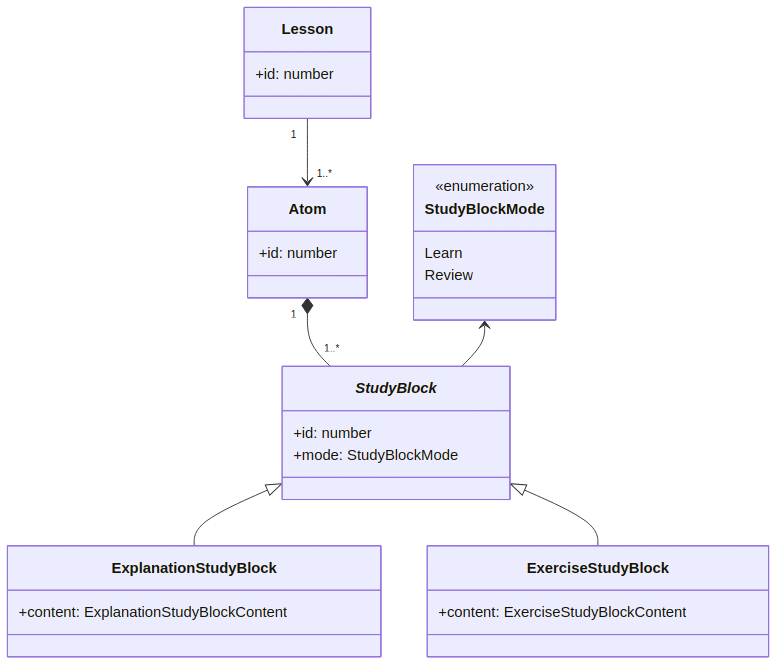
\includegraphics[width=\textwidth]{./images/diagrams/study-model.png}
        \caption{Základní model struktury učení}
        \label{fig:study-model}
    \end{minipage}
\end{figure}

% Final
\subsubsection{Průběh učení a opakování}

% Final
Při spuštění učení je uživateli zobrazena sekvence bloků učení, tedy bloků \texttt{ExplanationStudyBlock} a \texttt{ExerciseStudyBlock}, které jsou v módu \texttt{Learn}. Tento mód indikuje, že mají být bloky použity, pokud je látka pro uživatele nová a dříve se ji neučil. Uživateli je tak pro každý atom v lekci nejprve vysvětlena látka pomocí bloku \texttt{ExplanationStudyBlock}. Následně si uživatel látku procvičí pomocí bloku \texttt{ExerciseStudyBlock}. V rámci každé lekce se tak uživatel postupně naučí několik nových atomů. V průběhu učení aplikace sbírá data o tom, jak uživatel odpovídá v jednotlivých cvičeních. Na základě těchto dat je následně po dokončení lekce naplánováno opakování jednotlivých atomů v backendové části aplikace.

% Final
Pokud uživatel v rámci \texttt{ExerciseStudyBlock} cvičení odpoví špatně, aplikace mu nabídne možnost si zobrazit vysvětlení odpovědi a zkusit cvičení znovu. Pokud uživatel odpoví špatně třikrát po sobě, aplikace mu nabídne možnost daný blok s cvičením přeskočit.

% Final
Při spuštění opakování aplikace uživateli zobrazí pouze sekvence bloků \texttt{ExerciseStudyBlock}, které jsou označeny módem \texttt{Review}. Tyto bloky pomocí cvičení prověří, jak dobře si uživatel danou látku pamatuje. Bloky cvičení jsou vybrány v backendové části aplikace na základě toho, které atomy by si měl uživatel zopakovat podle plánovacího algoritmu. Na základě odpovědí uživatele jsou atomy opět po dokončení učení naplánovány k dalšímu opakování v backendové části aplikace.

% Final
\subsubsection{Vysvětlování látky pomocí \texttt{ExplanationStudyBlock}}

% Final
Vysvětlování látky pomocí \texttt{ExplanationStudyBlock} je tvořeno animacemi doplněnými o audio nahrávku vysvětlující danou látku. Stránky s vysvětlením látky tak připomínají krátká videa, díky kterým je uživateli vysvětlena látka před tím, než začne plnit jednotlivá cvičení. Klíčovým rozdílem oproti klasickým videím je způsob, jakým jsou tato videa vykreslována.

% Final
Na rozdíl od videí, která jsou například uložena ve formátu \texttt{mp4} a následně streamována přes internet, jsou komponenty těchto videí animovány v prohlížeči za běhu aplikace pomocí knihovny Remotion\footnote{Dostupné na: \href{https://www.remotion.dev/}{https://www.remotion.dev/}}. Tyto animace jsou vytvářeny na základě textového popisu videa v JSON formátu, který je obsažený v \texttt{ExplanationStudyBlockContent} v daném \texttt{ExplanationStudyBlock} bloku. Struktura obsahu videí je vyobrazena na diagramu \ref{fig:explanation-model} a budu se ji dále věnovat v následujících částech textu.

% Final
Výše popsaný přístup má několik zásadních výhod a také několik limitací.

% Final
Zaprvé, díky použité knihovně Remotion, která umožňuje snadno animovat UI komponenty za běhu aplikace, je možné snadno vytvořit knihovnu UI komponentů, které mohou být využity při vytváření vysvětlovacích videí. Protože knihovna Remotion pracuje s React komponenty, je možné komponenty videí vytvářet analogickým způsobem, jako zbytek UI komponentů v aplikaci, tedy s využitím zaběhlých jazyků a knihoven. Díky tomu lze v komponentech videí snadno aplikovat existující styly aplikace a zachovat tak naprosto konzistentní vzhled mezi samotnou aplikací a obsahem videí. Pokud bychom se například rozhodli změnit primární barvu nebo jiné styly v aplikaci, bude stejná změna automaticky aplikována ve všech vysvětlovacích videích. Vzhled videí tak bude vždy aktuální a konzistentní se vzhledem celé aplikace.

% Final
Se zmíněnými styly komponentů se pojí i další výhoda, která je spíše vedlejším efektem tohoto přístupu. Protože komponenty videí dodržují stejný styl jako zbytek aplikace, je ve videích reflektován i světlý a tmavý režim aplikace. Byť tento efekt nebyl primárním záměrem použitého přístupu, může výrazně zlepšit uživatelskou zkušenost při sledování videí. Pokud například uživatel preferuje používání aplikace v tmavém režimu při učení se večer, aplikace bude automaticky i všechna videa zobrazovat v tmavém režimu. Učení tak může být pro uživatele výrazně příjemnější.

% Final
Další výhodou je znovupoužitelnost komponentů uživatelského rozhraní. Pokud bychom například vytvořili v aplikaci komponent vizualizující algoritmus Bubble Sort, můžeme tento komponent využít jak v samotných cvičeních, tak ve vysvětlovacích videích. Tato znovupoužitelnost tak může zásadně zefektivnit tvorbu obsahu a zvýšit jeho kvalitu. Při tvorbě obsahu aplikace tak bude možné investovat více času do tvorby a testování jednotlivých komponentů a následně je využívat na více místech napříč cvičeními a videi.

% Final
Další kuriózní výhodou je responzivita samotných videí. Jelikož jsou videa tvořena responzivními UI komponenty, které jsou vykreslovány za běhu aplikace, je možné videa vytvořit tak, aby byly při dodržení určitých rozložení komponentů také responzivní. Videa je tak následně možné sledovat na zařízeních s různě velkými displeji, tedy na počítačích, tabletech i mobilních zařízeních. Docílení této responzivity samozřejmě nebylo přímočaré a bylo třeba zavést řadu opatření, aby byla videa skutečně responzivní. Tomuto tématu se budu podrobněji věnovat v následující podkapitole tohoto textu.

% Final
Kromě výše zmíněných výhod je další zásadní výhodou snadná udržovatelnost a rozšiřitelnost vysvětlovacích videí. Pokud například text ve videu obsahuje chybu nebo nepřesnost, stačí ji opravit v textové definici videa v \texttt{ExplanationStudyBlock} bloku v databázi. Uživatelům se pak začne ihned po načtení učení zobrazovat opravená verze videa. Tyto opravy se netýkají jen obsahu, ale i samotných komponentů videí. Pokud se například některý prvek videa zobrazuje chybně, jeho oprava bude po nasazení frontendu ihned reflektována ve všech vysvětlovacích videích. Tyto snadné změny se netýkají pouze chyb, ale i zdokonalování obsahu a jednotlivých komponentů videí. Díky tomu, že mohou být všechny změny takřka okamžitě aplikovány napříč celou aplikací, je tak možné velice efektivně vytvářet obsah aplikace a vylepšovat jeho kvalitu.

% Final
Poslední výhodou, kterou zde zmíním, je interaktivita samotných videí. Jelikož jsou komponenty videí vykreslovány dynamicky a jedná se o UI komponenty, je možné docílit různých interaktivních efektů. Ve videích je tak možné například vykreslit tlačítko, které bude reagovat na kliknutí uživatele. Jiný komponent může zase například vykreslit aktuální počasí na určitém místě. Byť jsem v rámci této práce do videí žádné interaktivní komponenty nezahrnoval, bude možné v budoucnu videa rozšířit tak, aby byly interaktivnější a poutavější.

% Final
S výše zmíněnými výhodami tohoto přístupu se pojí několik limitací, které je třeba brát v úvahu. Jelikož jsou animace vytvářeny za běhu aplikace v prohlížeči, je třeba brát v potaz výkon prohlížečů, použitých programovacích jazyků a výkon samotných zařízení uživatelů. Prohlížeče s jazykem JavaScript ze své podstaty nebyly vytvořeny primárně pro dynamické vykreslování komplexních videí. Uživatelé mohou také používat aplikaci na různě starých a výkonných zařízeních, což může limitovat schopnost prohlížeče přesně v daném čase animovat jednotlivé komponenty. Kvůli těmto limitacím by bylo nepraktické využívat tento způsob vykreslování pro složitější a graficky náročnější animace. Pokud by například bylo třeba vykreslit vizualizaci nějaké simulace, v níž by se pohybovalo přes deset tisíc prvků, byl by tento přístup takřka nepoužitelný.

% Final
Z výše zmíněného důvodu jsem se rozhodl vytvořit komponent \texttt{Video}, díky kterému je možné do vysvětlovacích videí vložit video ve standardním formátu, tedy například ve formátu \texttt{mp4}. Díky tomu lze kombinovat oba výše zmíněné přístupy. Pro definici struktury videa je tak možné použít přístup popisovaný v této kapitole a pro složitější vizualizace lze na některých místech využít zmíněný komponent \texttt{Video}.

% Final
Další limitací rozebíraného přístupu je responzivita samotných videí. Pokud chceme docílit responzivity videí, je třeba zásadně přizpůsobit rozložení prvků mobilním zařízením, které mají na displeji, ve srovnání s ostatními zařízeními, výrazně méně prostoru. Aby bylo dosaženo plně funkční responzivity, je třeba zásadně zjednodušit strukturu videí a zredukovat tak počet zobrazovaných komponentů, které lze v jednu chvíli ve videu zobrazit. Této responzivitě se budu věnovat v následující podkapitole tohoto textu.

% Final
Poslední limitací, kterou zde zmíním, je použitelnost videí v situacích, kdy uživatel nemá možnost poslouchat audio. Pokud například uživatel jede v autobuse a nemá k dispozici sluchátka, jeho možnost sledovat vysvětlovací videa je značně limitována. Tato limitace vychází spíše z rozhodnutí vysvětlovat látku formou videí, než ze samotného přístupu vykreslování videí. Byť je tato limitace zásadní z hlediska uživatelské zkušenosti, je cenou za získání potenciálně záživnější formy výuky a názornějšího vysvětlování látky.

% Final
Výše zmíněnou limitaci jsem se snažil minimalizovat tím, že jsem k videím implementoval možnost si zobrazit titulky, pokud uživatel nemá možnost poslouchat audio. Uživatelé, kteří nemají možnost poslouchat audio, si tak aspoň mohou při sledování videa číst titulky a získat tak informace touto cestou.

% Final
Celkově tak tato forma vysvětlování látky má několik zásadních výhod a limitací. V rámci této práce jsem došel k názoru, že zmíněné výhody převažují nad nevýhodami a rozhodl jsem se tak v této práci popsaný přístup použít.

% Final
\subsubsection{Responzivita videí s vysvětlením látky}

% Final
V této části textu popíšu, jakým způsobem jsem zajistil responzivitu vysvětlovacích videí, kterou jsem zmínil v předchozí kapitole.

% Final
Aby bylo docíleno responzivního chování videí, bylo třeba, aby videa dodržovala jednoduchou a přesně danou strukturu. Z tohoto důvodu jsem zavedl následující strukturu videí. Každý \texttt{ExplanationStudyBlockContent} se skládá z několika scén \texttt{Scene}. Každá scéna se pak skládá ze stránek \texttt{Slide}, které významově odpovídají stránkám v prezentacích. Každý \texttt{Slide} je pak rozdělen do jednoho až tří sloupců \texttt{Column}, ve kterých jsou následně zobrazovány jednotlivé komponenty. Komponenty ve sloupcích se vždy zobrazují pod sebou v pořadí, ve kterém jsou ve sloupci zadefinovány. 

% Final
Pro zjednodušení tvorby stránek ve videích jsem dále zavedl dva typy stránek. Prvním typem je \texttt{RawSlide}, který umožňuje přesně definovat, které komponenty se mají na stránce zobrazit. Druhým typem je \texttt{SlideTemplate}, který je možné dále rozšiřovat a vytvářet tak předpřipravené šablony stránek. Tyto šablony poskytují oproti \texttt{RawSlide} stránkám zapouzdření jednotlivých komponentů a jednodušší rozhraní. Šablony je tak možné využívat pro efektivnější tvorbu videí. Popsaný model je vyobrazen na diagramu \ref{fig:explanation-model}.

% Review - přizpůsobit textwidth tak, aby se to vešlo do diplomky
\begin{figure}[!h]
    \centering
    \begin{minipage}{0.9\textwidth}
        \centering
        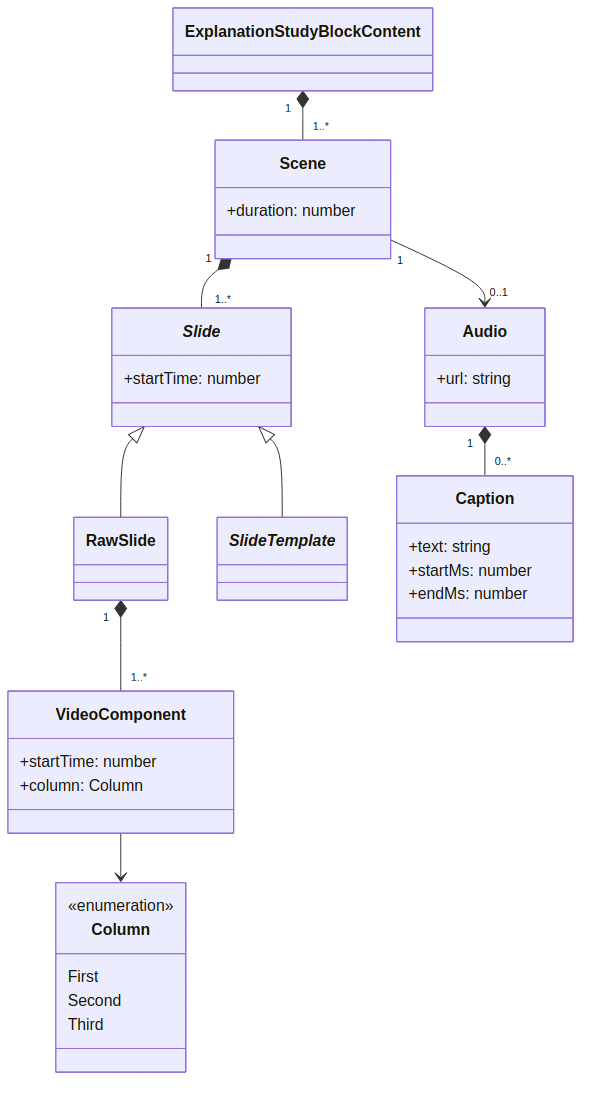
\includegraphics[width=\textwidth]{./images/diagrams/explanation-model.png}
        \caption{Základní model videí s vysvětlením látky}
        \label{fig:explanation-model}
    \end{minipage}
\end{figure}

% Final
Na širokých displejích, tedy například na monitorech nebo mobilních zařízeních orientovaných na šířku, jsou jednotlivé sloupce vykreslovány vedle sebe. Pokud uživatel ovšem sleduje video na zařízení s úzkým displejem, tedy typicky na mobilním zařízení otočeným na výšku, jsou pak sloupce vykreslovány pod sebou. Jednotlivé komponenty se dále přizpůsobují dostupnému místu, podobně jako responzivní komponenty na webových stránkách. Tento systém tak umožňuje snadno umisťovat komponenty na obrazovku tak, aby se jejich rozložení přizpůsobovalo velikosti a orientaci obrazovky.

% Final
Limitací tohoto přístupu je množství komponentů, které je možné ve videu na jedné stránce zobrazit. Do sloupců například není vhodné umisťovat přehršel komponentů s pevně danou výškou, protože by se z důvodu přesunu sloupců na menších displejích pod sebe jednotlivé komponenty nevešly. V důsledku by videa měla být tvořena tak, aby obsahovala více jednodušších stránek s méně komponenty, než méně stránek s mnoha komponenty. Dále, pokud je například třeba zobrazit komplexnější komponent, který obsahuje více detailů nebo textu, je vhodné na obrazovce zobrazit pouze tento komponent v jednom sloupci. Díky tomu bude mít sloupec na všech velikostech displeje maximální výšku a šířku a komponent tak bude možné lépe vidět.

% Final
Samotné komponenty bylo také třeba vytvářet s ohledem na responzivitu videí. Například komponenty zobrazující kód jsem implementoval tak, aby bylo možné při jejich použití určit, v jaké fázi videa se má zobrazit jaká část kódu. Pokud by tak například bylo třeba ve videu ukázat kód s mnoha řádky a vysvětlovat různé části tohoto kódu, je možné v definici komponentu označit jednotlivé části, o kterých se bude ve videu ve vybraném čase mluvit. Aplikace pak bude automaticky v daném čase scrollovat na specifikovanou část kódu, díky čemuž bude moci uživatel vždy na obrazovce vidět, o které části kódu je ve videu řeč.

% Final
\subsubsection{Plnění cvičení pomocí \texttt{ExerciseStudyBlock}}

% Final
Po tom, co byla v rámci učení uživateli vysvětlena látka pomocí dříve popsaných bloků s vysvětlením látky \texttt{ExplanationStudyBlock}, jsou uživateli zobrazeny bloky \texttt{ExerciseStudyBlock}, které slouží k procvičení dané látky a sběru dat o tom, jak uživatel dané látce rozumí.

% Final
Každý tento blok je, podobně jako bloky s vysvětlením látky, vykreslen na samostatné stránce v rámci učení. Tento blok může obsahovat jeden nebo více komponentů \texttt{ExerciseStudyBlockComponent}, které jsou vykresleny pod sebou v jednom sloupci. Komponenty jsou buď pasivní, které pouze zobrazují informace, nebo aktivní, se kterými může uživatel interagovat. Pasivní komponenty jsou například nadpisy, odstavce nebo diagramy. Aktivními komponenty jsou různá cvičení, které musí uživatel vyplnit pro splnění daného bloku. Jeden \texttt{ExerciseStudyBlock} může obsahovat více aktivních komponentů. Příkladem toho je editor kódu, který obsahuje více oken s kódem. Každé okno je pak považováno za samostatný komponent cvičení.

% Final
Po vyplnění všech aktivních komponentů v rámci daného bloku uživatel zvolí možnost zkontrolovat výsledky, aplikace odpověď ohodnotí a zaznamená. Uživatel má pak možnost pokračovat nebo odpověď opravit v případě, že byla špatná.

% Final
Podobně jako bloky s vysvětlením látky, mohou bloky se cvičeními obsahovat audio nahrávku, která doprovází uživatele při učení. Na rozdíl od bloků s vysvětlením látky, kde je audio nahrávka přehrávána v rámci celého videa, je v případě bloků se cvičeními audio nahrávka pouze připojena ke konkrétním komponentům. Každý komponent tak k sobě může mít připojenou audio nahrávku, která například vysvětluje zadání daného příkladu. Po načtení \texttt{ExerciseStudyBlock} bloku se postupně přehrají všechny audio nahrávky, které jsou v komponentech daného bloku obsaženy. Díky tomu například uživatel nemusí číst text se zadáním, ale může si ho poslechnout a následně hned vyplnit dané cvičení.

% Final
Díky audio nahrávkám a flexibilní struktuře bloků cvičení a vysvětlování látky je tak možné pro uživatele vytvářet vysoce interaktivní průchody učením a opakováním. Způsob výuky v této aplikaci se tak blíží interaktivním lekcím konkurenčních aplikací Scrimba a Mimo, které jsem analyzoval v rámci analýzy existujících řešení.

% Write - tuhle sekci sepsat
\subsection{Push Notifikace}

% Review
\subsection{Přizpůsobení aplikace pro PWA}

% Review
V rámci nefunkčního požadavku jsem doplnil konfiguraci aplikace nutnou pro to, aby prohlížeče aplikaci klasifikovaly jako progresivní webovou aplikaci. V souboru \texttt{manifest.ts} jsem definoval metadata aplikace, jako například název, jazyk aplikace, základní barvy a ikony. V rámci této konfigurace jsem také vytvořil několik základních ikon, které může progresivní webová aplikace využívat.

% Review
Dále jsem do aplikace doplnil registraci tzv. Service Worker služby. Service Worker je skript běžící v prohlížeči, jehož životní cyklus je takřka nezávislý na životním cyklu aplikace. Service Worker tak může běžet ve vlastním vlákně nezávisle na samotné aplikaci. Tato služba se využívá například pro správu cache aplikace, podporu offline funkcí a jako proxy mezi odchozími a příchozími požadavky a samotnou aplikací. V rámci této práce jsem se těmto funkcím nevěnoval a proto jsem pouze zaregistroval prázdný Service Worker skript, který je nutný pro vytvoření PWA. \cite{ServiceWorker}

% Review
Nakonec bylo třeba zajistit, aby byla aplikace dostupná přes HTTPS protokol \cite{PWABuilder}. To jsem zajistil v rámci nasazení aplikace, kterému se věnuji v podkapitole \nameref{sec:deployment}.

% Review
Díky výše zmíněné konfiguraci se tak aplikace stala progresivní webovou aplikací. Uživatelé si tak mohou aplikaci stáhnout a nainstalovat do svých zařízení přímo z prohlížeče na stránkách této aplikace.

% Review
Aplikaci tak bude možné v budoucnu po dalších konfiguracích, například s pomocí nástroje PWABuilder \cite{PWABuilder}, zabalit a publikovat na platformách Google Play, App Store nebo například Microsoft Store. Publikace na tyto platformy je časově značně náročná a týká se spíše právních otázek, nežli softwarového inženýrství. Proto se samotné publikaci v rámci této práce nebudu věnovat.
